\documentclass[12pt]{article}

%PACKAGES
\usepackage{graphicx}
\usepackage{epstopdf}
\usepackage[english]{babel}
\usepackage[toc,page]{appendix}
\usepackage{caption}
\usepackage{subcaption}
\usepackage{listings}
\usepackage{subfig}
\usepackage{multicol}

\usepackage{hyperref}
\usepackage[left=3cm,top=3cm,right=3cm,nohead,nofoot]{geometry}
\usepackage{braket}
\usepackage{datenumber}
\usepackage{placeins}


%COMMANDS

\begin{document}

\begin{center}
\Huge
Detection of galaxies superclusters in simulated cosmological structures\\  
\vspace{3mm}
\Large Sergio Daniel Hern\'{a}ndez Charpak

\large
200922618

\vspace{2mm}
\Large
Advisor: Jaime E. Forero-Romero

\normalsize
\vspace{2mm}

\today
\end{center}


\normalsize
%\newpage
\tableofcontents
\newpage

\section{Abstract}
Recently Tully et al. (2014) \cite{tully_laniakea_2014} used local cosmic flow information to
define our local supercluster, Laniakea. 
In this work we present a study on large cosmological N-body
simulations aimed at establishing the significance of Laniakea in a
cosmological context.
We explore different algorithms to define superclusters from the dark
matter velocity field in the simulation. 
We summarize the properties of the supercluster population by their
abundance at a given total mass and its shape distributions.
We find that superclusters similar in size and structure to Laniakea are
relatively uncommon on a broader cosmological context.
We finalize by discussing the possible sources of systematics (both in
our methods and in observations) leading to this discrepancy.

\section{Introduction}

In the Universe scene at large scales the galaxies group themselves in structures
similar to a filament web which go through large voids regions and cross in regions
called superclusters. Even though these structures can be easily detected at simple
view, there are different possibilities to delimited them from physical criteria \cite{gott_iii_map_2005}.    
\\

A proposal to define a supercluster is to use the flow of galaxies in this region of
space. Within a supercluster, galaxies tend to flow to the most dense region as a
consequence of the gravitational attraction process. In this way, spacial regions where
the galaxy flow is convergent represent galaxies superclusters.\\
\\
Recently a team build a galaxies velocities flow map of the local group in a scale of
hundreds of light years \cite{tully_cosmicflows-2_2013}. In this map converging points
were found and this team identified Laniakea, the galaxies supercluster which includes
our galaxy, the milky way \cite{tully_laniakea_2014}.
\\   

We propose to develop a method to detect a statistical significant number of galaxies
supercluster in cosmological simulations. 
With this we aim to quantified if Laniakea can be considered as an atypical structure in
the Universe. 
\\

\section{Background}
\subsection{Cosmic flows and peculiar velocities}
%Describe in detail the Laniakea work and the Methods used
The peculiar velocity refers to the velocity relative to a rest frame. In the case of the
Cosmicflows-2 map, the rest frame is the earth. 
The Laniakea supercluster of galaxies was mainly identified following an analysis of the
peculiar velocities flows. A Wiener filtering method was apply to obtained a better
Signal/Noise proportion and separate the peculiar velocities from the cosmic expansion.\\
%Explain how the fieltering worked
This is to be explained in further detail.



\subsection{Boundaries of Laniakea}
The contour of the region were reconstructed with the V-web Algorithm. This algorithm is deeply connected to the velocities as its core is the shear velocity tensor.\\

%Explain how the V-Web algorithm worked. 
This is to be explained in further detail.

\section{Methods}

As we support the open-source community, we used the N-Body simulation open
software Gadget-2 \cite{springel_gadget_2_2005} to generate the simulations
and source code in C and Python to treat the data obtained from the
simulations. The development of the code will be in Github \url{https://github.com/sercharpak/Monografia/}.

\subsection{Simulations}
We used the N-Body simulation software Gadget-2 \cite{springel_gadget_2_2005}
widely used in the scientific community to generate a box of size 500 Mpc/h
with $512^{3}$ dark matter particles (DM). The initial conditions were
generated with Springel's N-Genic software. The simulations ran on the HPC cluster at UNIANDES with 48 processors and took approximately 10 hours to run. \\

By DM particle we mean a particle which only interacts through gravity
interaction. In the simulation each particle represents a galaxy. The DM particles are
placed in a 3D grid layout first and then are perturbed following Poisson distribution
before the simulation start, during the initial conditions generation.\\

Once the simulation starts, the particles interact only with gravity as time goes by following the cosmological constants. Here these were not modified, the default values were used.\\

We then use different algorithms to identify the superclusters within the simulation.\\

\subsection{Approach and Algorithms}

So far we have used a naive way to approach to the problem. 
\begin{enumerate}
	\item We calculate the magnitude of the velocity (the speed) of each particle. 
	\item We look for regions where the center has the highest speed and from it the speed decreases while the particle is further away from the center. 
    \item We define the limits of this region the regions where the speed begins to increase with the distance from the center.
\end{enumerate}

We used a region growing algorithm, a simple image segmentation algorithm
used to identify different regions in a image \cite{gonzalez_digital_2008}.\\
$f(x,y,z)$ denotes the input data. $S(x,y,z)$ denotes a seed array, with
value 1 where the particle can be define as a seed and 0 where not. It is the
same size of $f(x,y,z)$. $Q$ denotes a predicate which is to be apply to the
input data and determines if the region which starts at the seeds grows or
not. Here $Q$ denotes: "if the speed of the close particle is lower than the
marked one but greater than a threshold, mark that particle and continue."

\begin{enumerate}
	\item We choose seeds to begin the growth. In this case we choose the particles with high velocities. Here \[ |v|>  th_{high}\]
	\item We open a window of particles to look for 2 close particles from the seed $s$ which do not for part of $S(x,y,z)$. Here:
    \[ window = 20000\]
    \item Once we found the 2 close particles $c$ we apply the predicate $Q$. Here:
    \[ Q := |v_s| > |v_c| > |th_{low}|\]
    
    \item If the particle $c$ satisfies $Q$, it is marked, $S(c) = 1$
    \item Apply the algorithm to $c$, and so on (Recursion).
\end{enumerate}

Here we defined empirically different thresholds in order to observer the results. \\
First we used:  \\
$th_{low} = v_{min} + \frac{\sigma_{v}}{2} $ and $th_{high} = v_{max}  - \sigma_{v}$ .\\
Secondly we used: \\
$th_{low} = \bar{v} + 2  \sigma_{v} $ and $th_{high} = \bar{v}  +  8 \sigma_{v}$.\\

The first version of the algorithm was written in python using the module
pyGadgetReader \cite{thompson_pygadgetreader_2014ascl_soft11001T} to read the
data and transform it to NumPy arrays in Python. In Appendix \ref{App:AppendixA} we attach the source code used.


\section{Results}

The simulation ran correctly on 48 processors in approximately 10 hours. We first visualized the simulation and its distribution of velocities. \\

We first visualize the speed histogram.\\

%Speed histogram
\begin{figure}[ht]
\begin{center}
\includegraphics[width=0.9\textwidth]{graphs/hist_vel.png} % Include the image placeholder.png
\caption{Speed Histogram of the simulation}
\label{fg:hist_vel}
\end{center}
\end{figure}
\FloatBarrier

The histogram resemble a Poisson distribution. This is a consequence of the perturbations generated in the initial conditions generation. 

\begin{table}[ht]
    \centering
    \begin{tabular}{|c|c|}
        $v_{max}$ & 2023.87 \\
        $v_{min}$ & 0.34\\
        $\sigma_{v}$ & 117.75 
    \end{tabular}
    \caption{Properties of the speed distribution}
    \label{tab:vel}
\end{table}
\FloatBarrier


Our hypothesis is based on the most direct implication of gravity. The lower speed
particles will mainly be in the border regions and the higher speed particles
will be in the center regions. \\

For this we must choose a threshold for low velocities and a threshold for high velocities. 
We obtain: $th_{low} = v_{min} + \frac{\sigma_{v}}{2} = 59.2$ and $th_{high} = v_{max}  - \sigma_{v} = 1906.12 $

%Plot 3Ds
%First 3D plot, particles with speed lower than thresh_low
We first have a look at the particle distribution of particles with speed higher than the
threshold for low velocities.\\
%59.216707265
\begin{figure}[ht]
\begin{center}
\includegraphics[width=0.8\textwidth]{graphs/pos_3d_vel_menor_s_smaller.png} % Include the image placeholder.png
\caption{DM particles with $|v| < 59.2 $}
\label{fg:3d_thresh_low}
\end{center}
\end{figure}
\FloatBarrier

There seem to be some structures, but it is not clear enough. This is due to the high number of DM particles used in the simulation ($512^3$). 

%Second 3D plot, particles with speed higher than thresh_high

We produce cuts in the z-direction to visualize in 2-D the speed distribution. \\

%Plot 2D

%5 plots of the 2D. 
%\begin{figure}[ht]
%\centering
%\begin{minipage}{.15\textwidth}
%  \centering
%  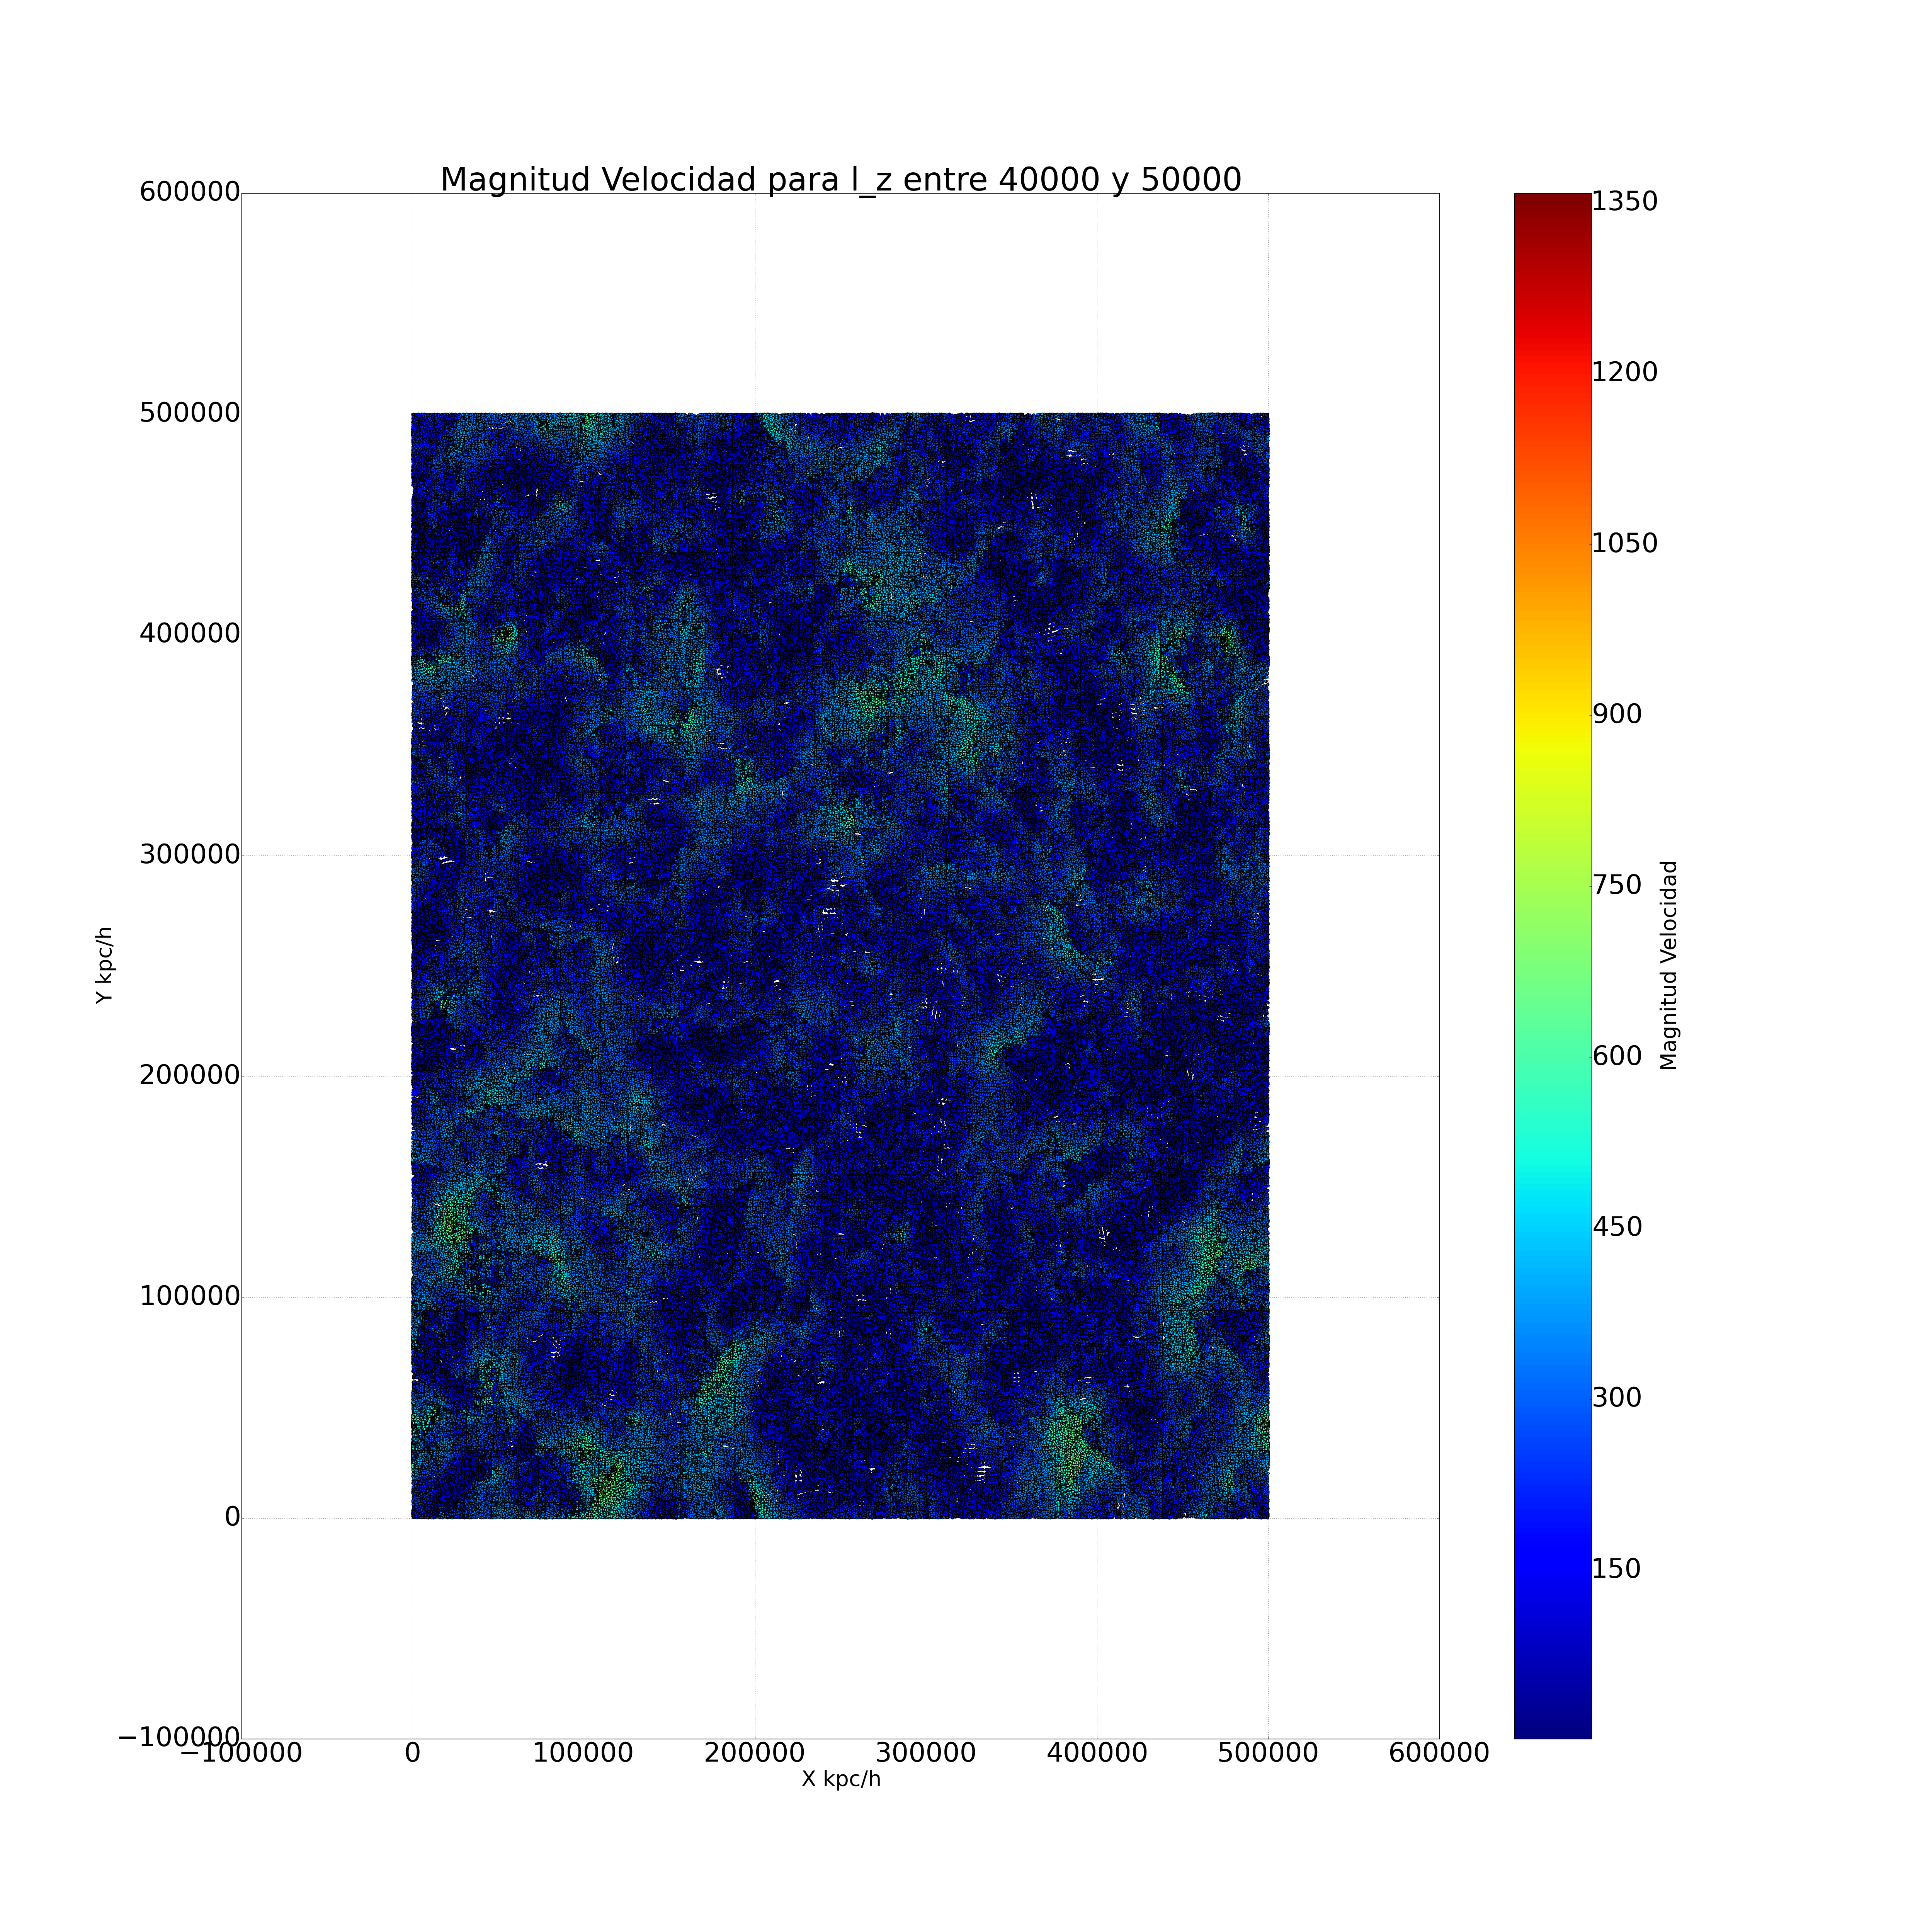
\includegraphics[width=0.2\textwidth]{graphs/scatter_magnitud_vel50000.png}
%\end{minipage}%
%\begin{minipage}{.15\textwidth}
%  \centering
%  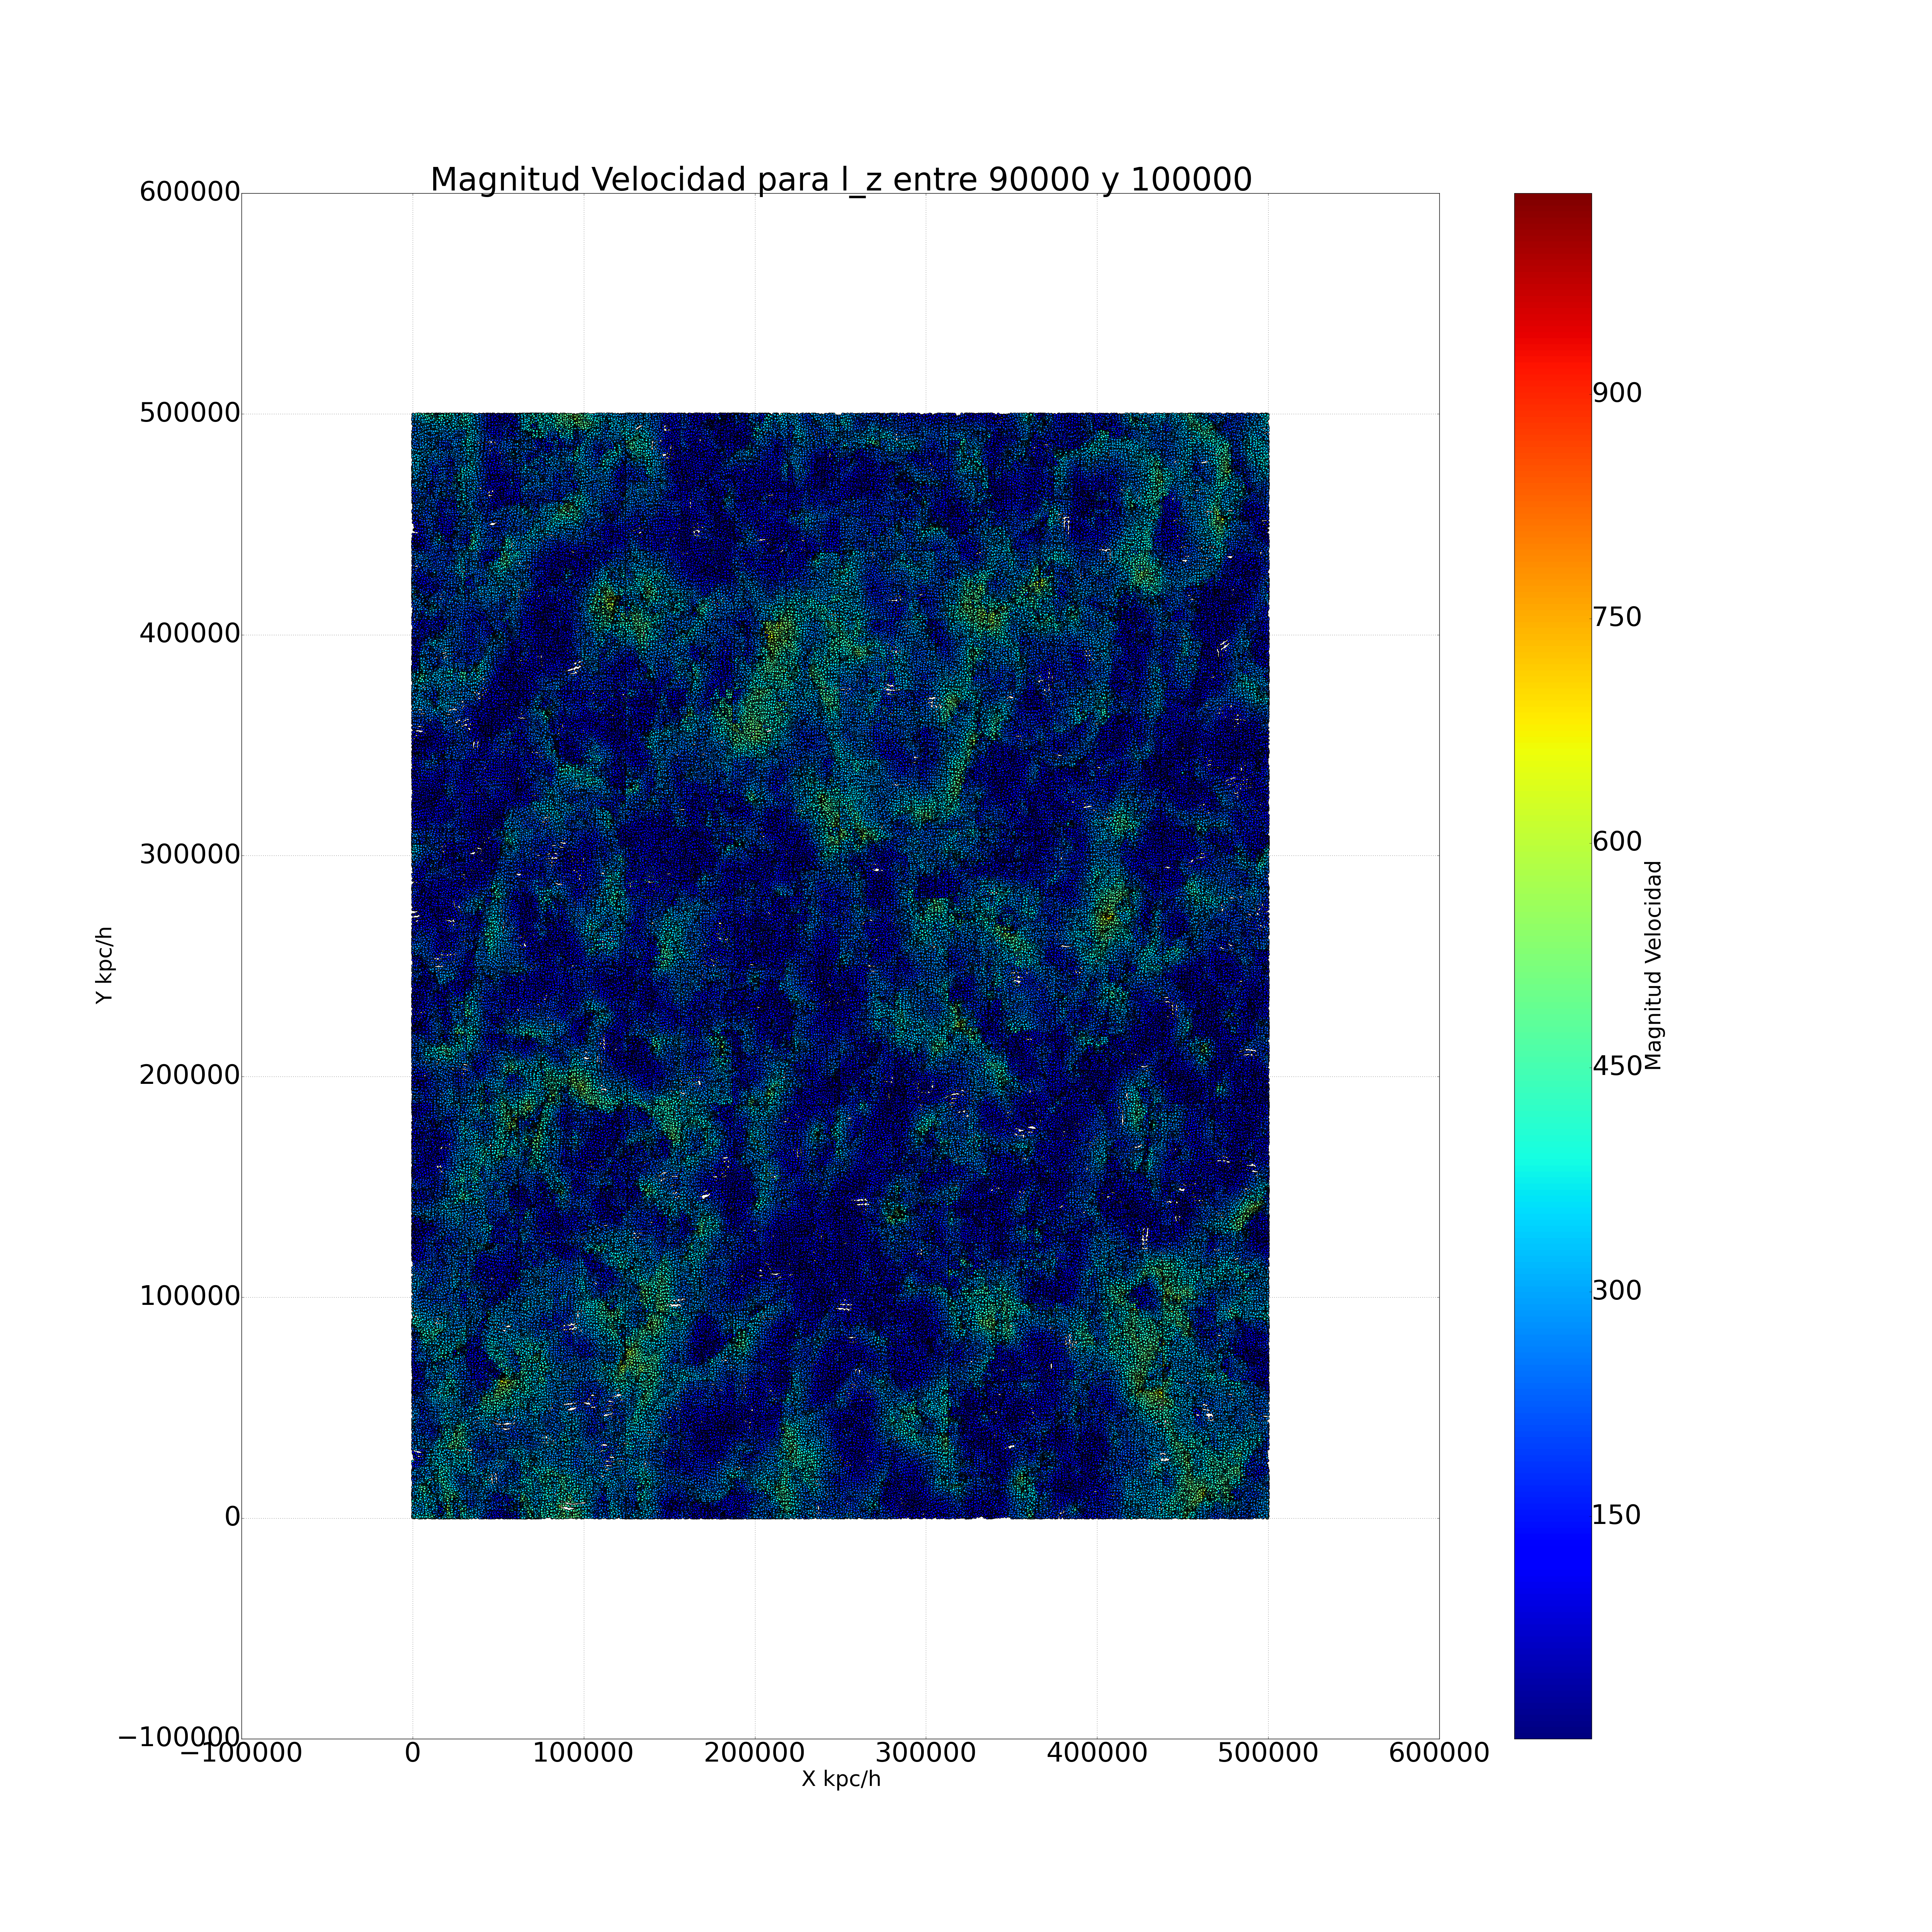
\includegraphics[width=0.2\textwidth]{graphs/scatter_magnitud_vel100000.png}
%\end{minipage}
%\begin{minipage}{.15\textwidth}
%  \centering
%  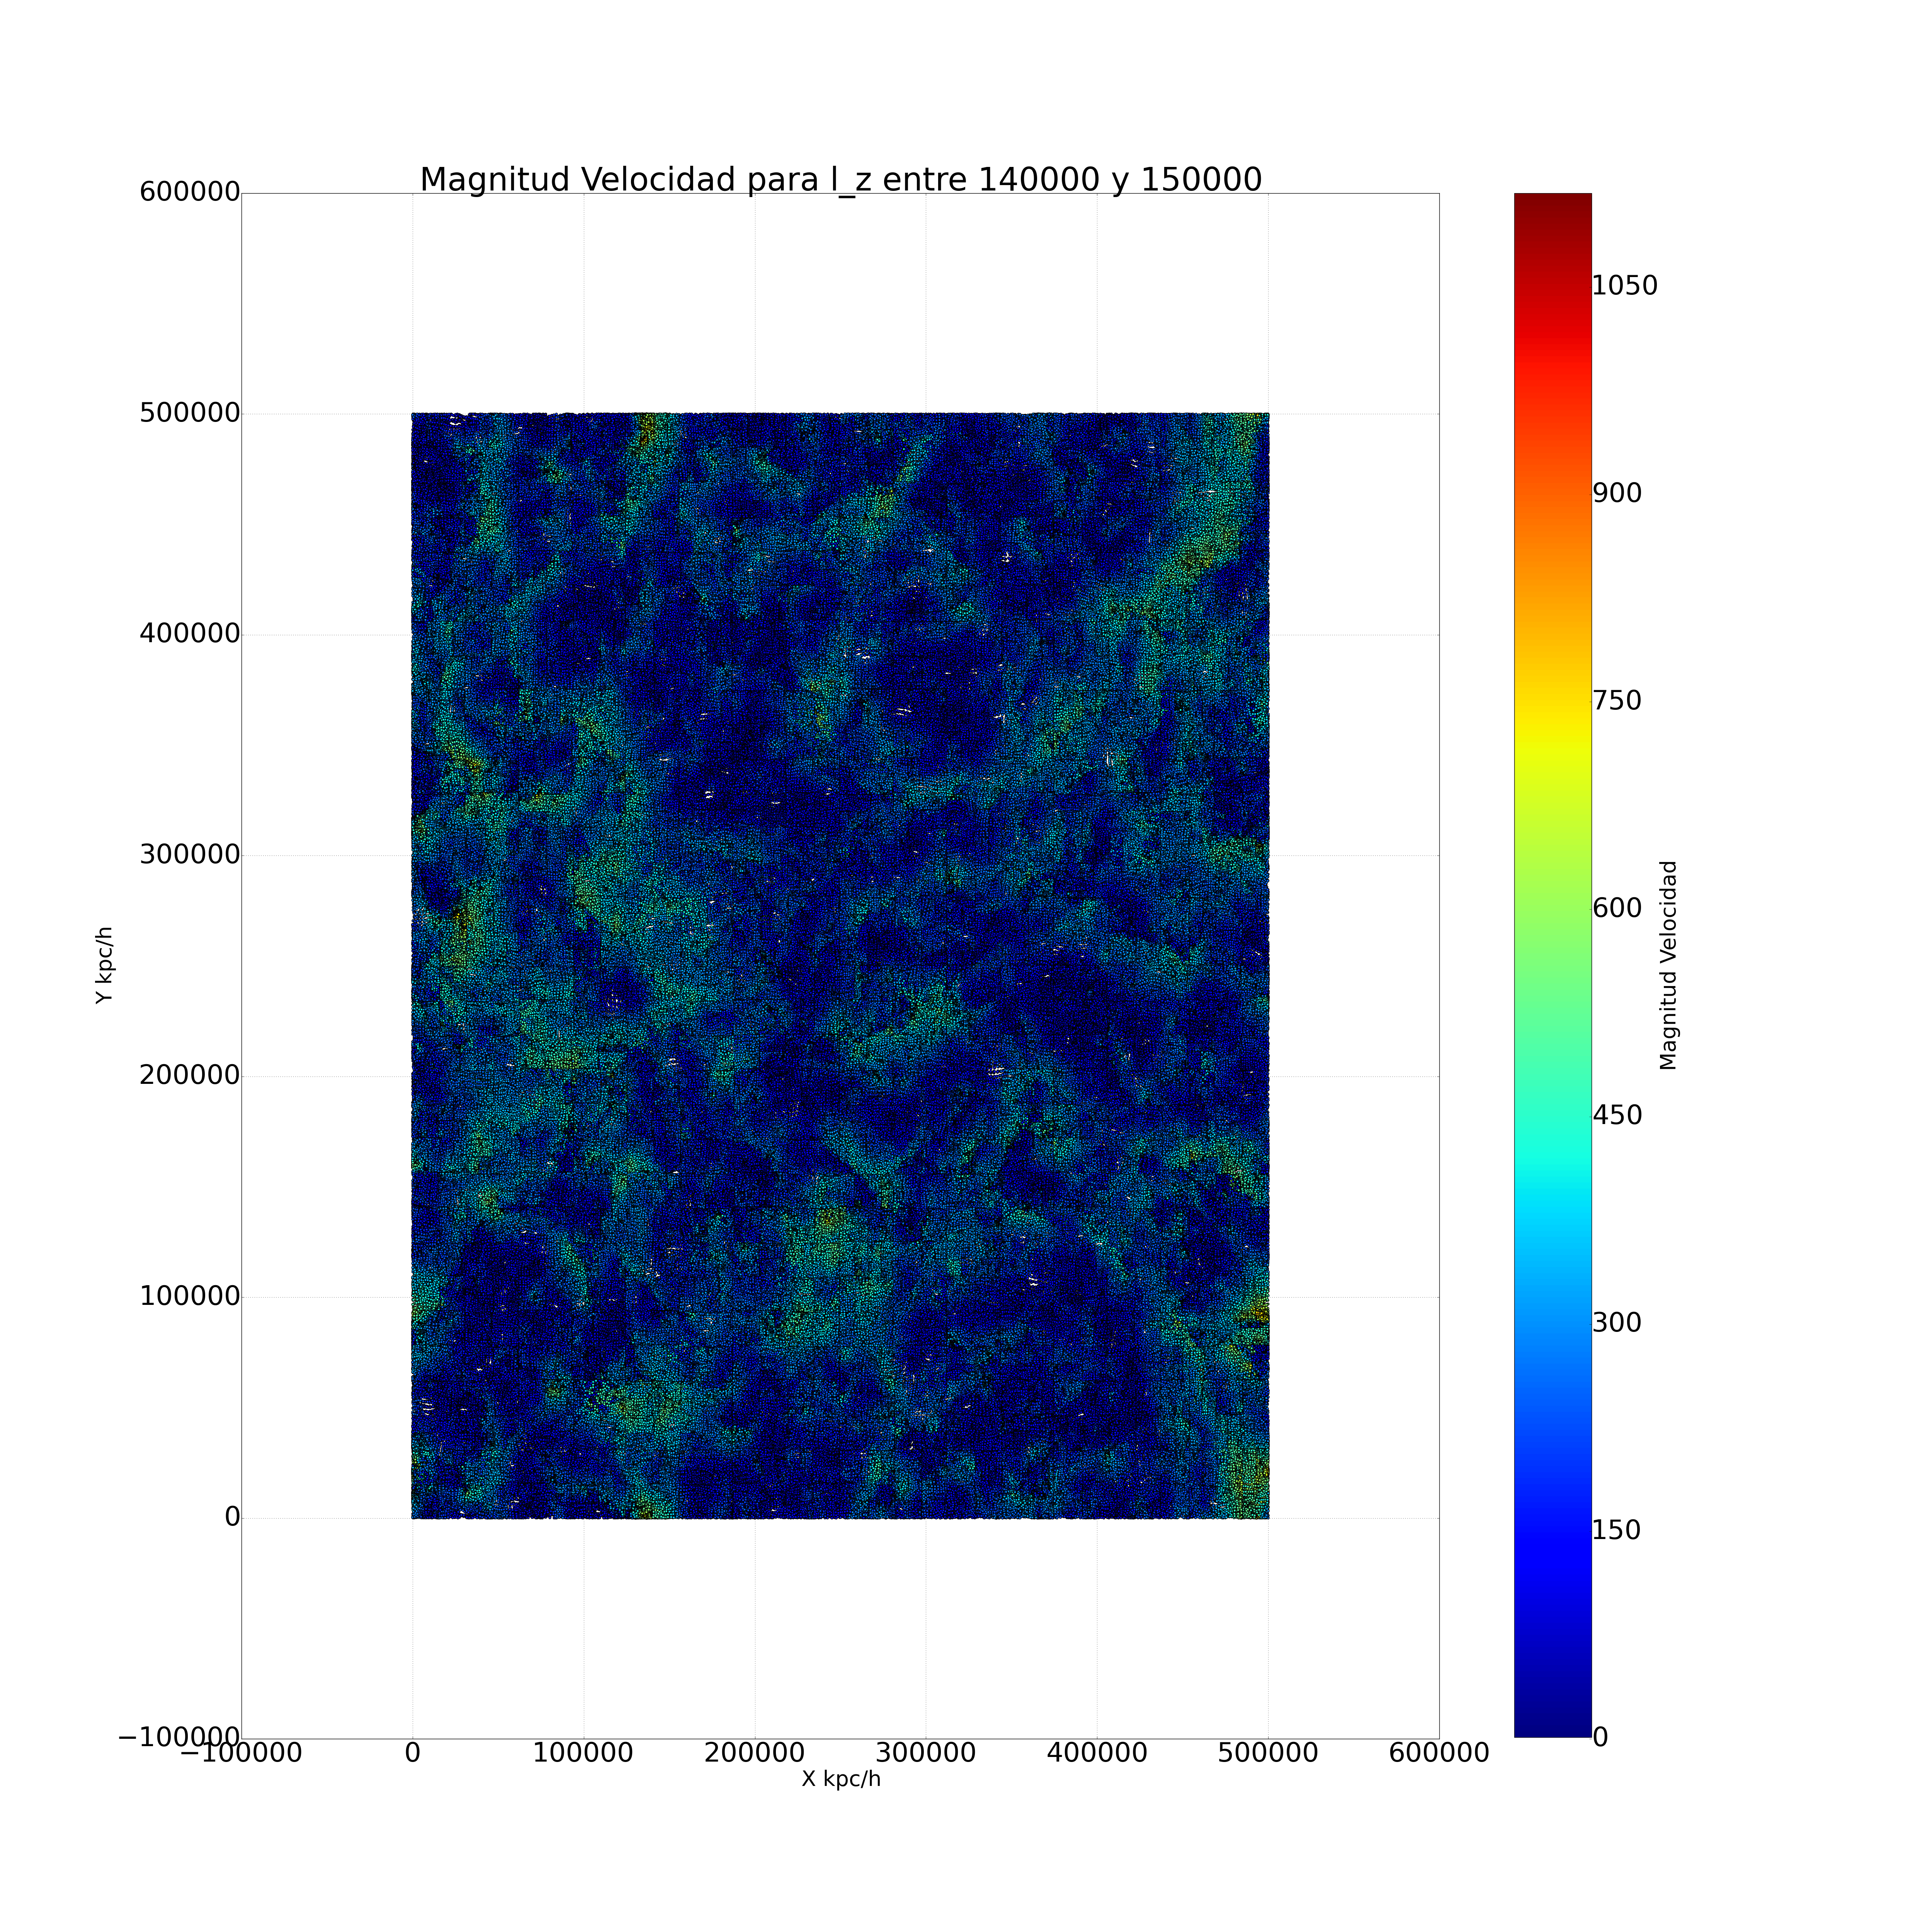
\includegraphics[width=0.2\textwidth]{graphs/scatter_magnitud_vel150000.png}
%\end{minipage}
%\begin{minipage}{.15\textwidth}
%  \centering
%  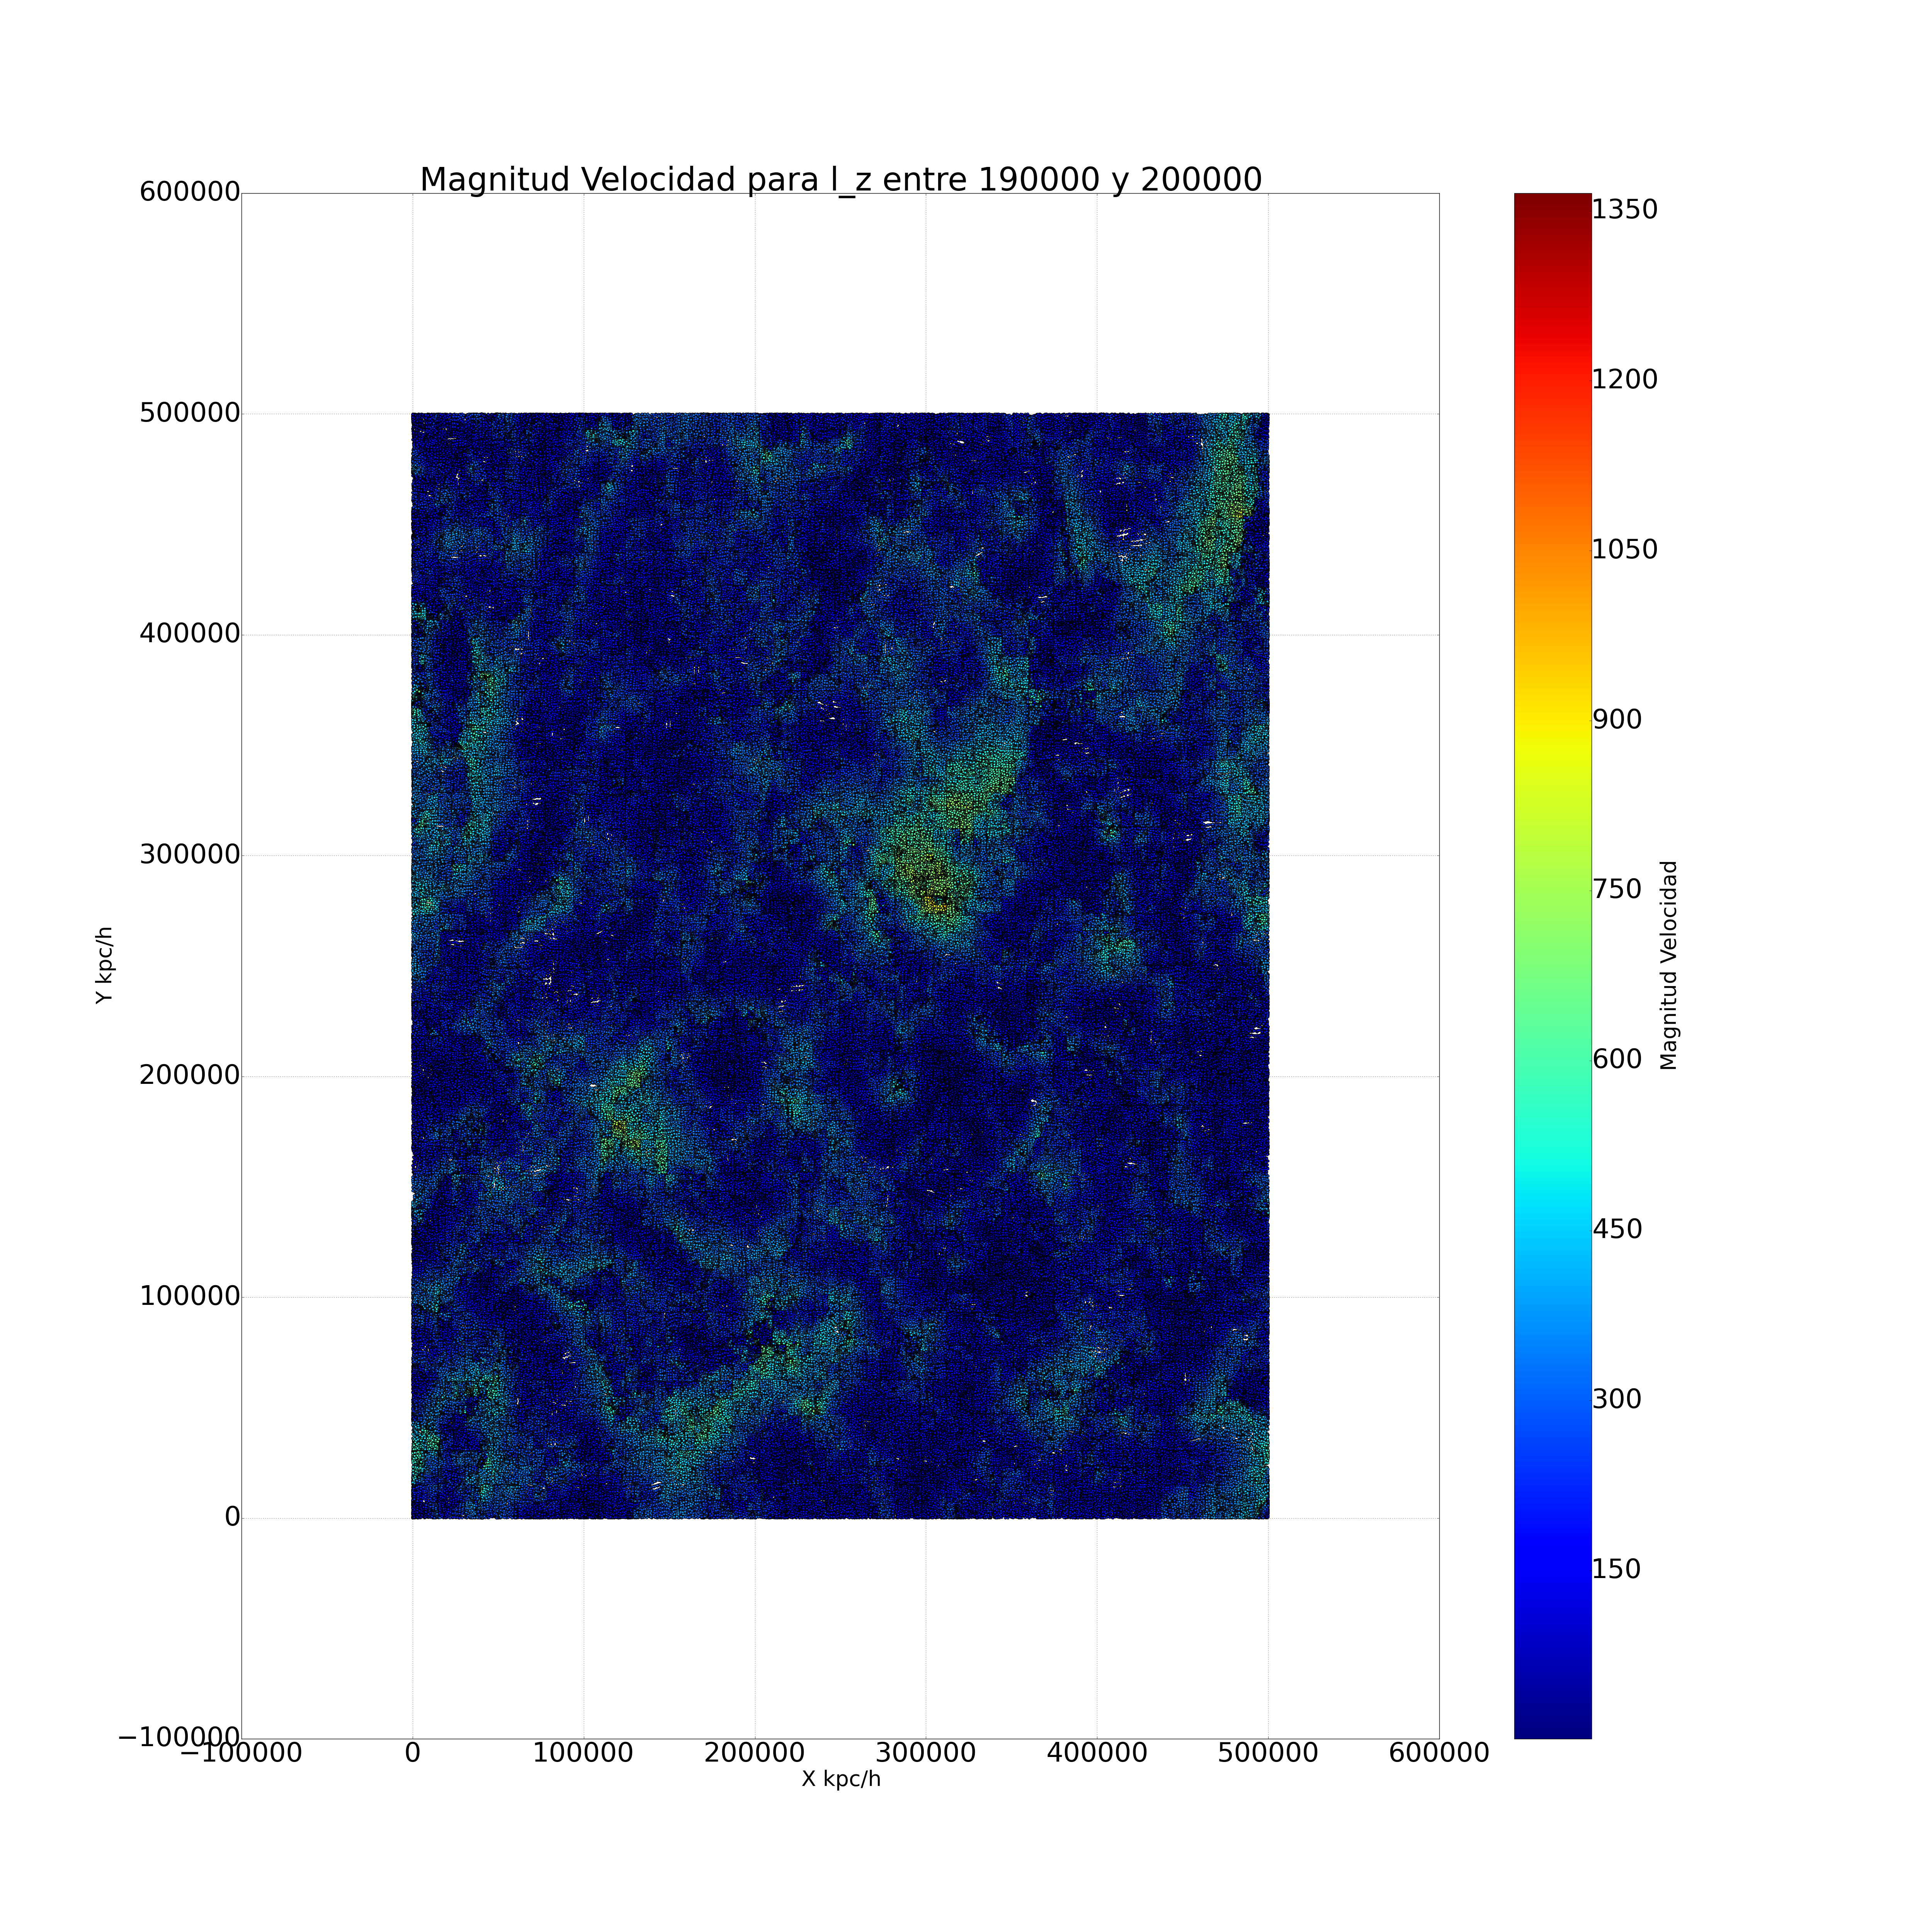
\includegraphics[width=0.2\textwidth]{graphs/scatter_magnitud_vel200000.png}
%\end{minipage}
%\begin{minipage}{.15\textwidth}
%  \centering
%  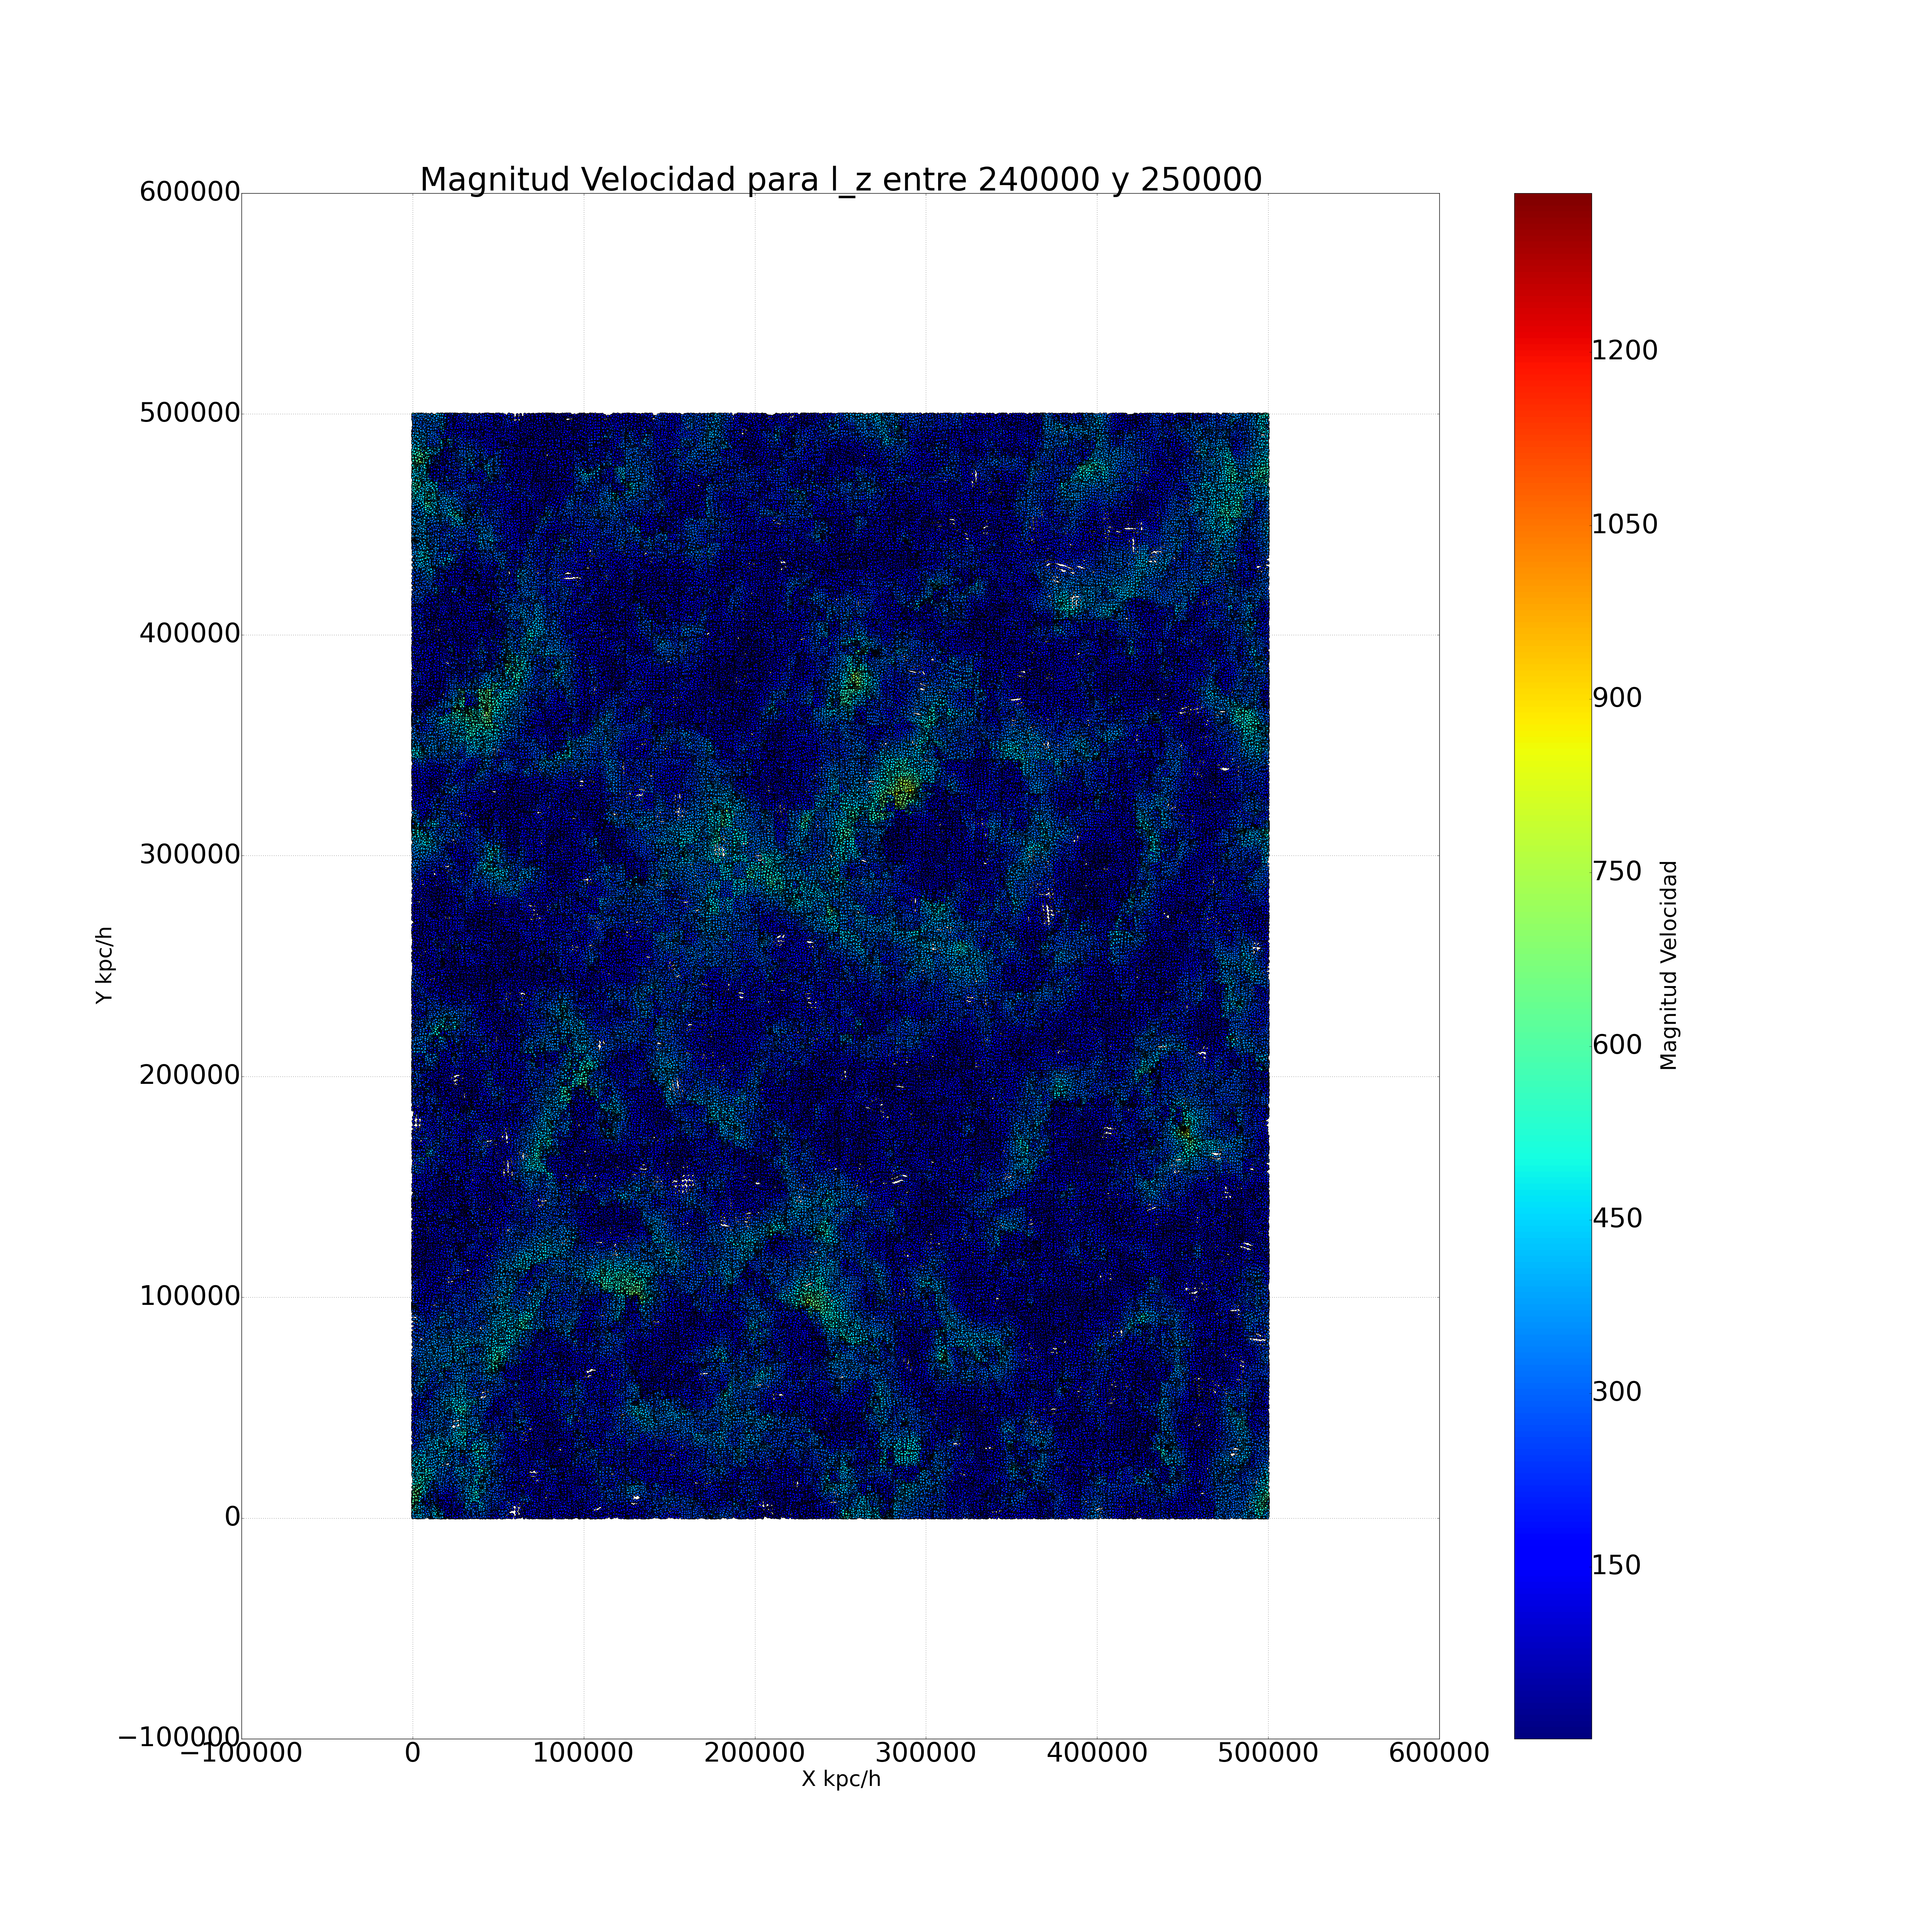
\includegraphics[width=0.2\textwidth]{graphs/scatter_magnitud_vel250000.png}
%\end{minipage}
%\caption{2D slices of the speed distribution}\label{fig:2D_slices}
%\end{figure}
%\FloatBarrier


We can observe more intuitive signs of structures related to the speed distribution. 
We can observe filament structures\\

It is more clear if we observe from one side the particles with speed greater than $th_{high}$ and the particles with speed lesser than $th_{low}$.\\

%\begin{figure}[ht]
%\centering
%\begin{minipage}{.2\textwidth}
%  \centering
%  \includegraphics[width=0.2\textwidth]{graphs/scatter_magnitud_vel_488_lz_100000.png}
%\end{minipage}%
%\begin{minipage}{.2\textwidth}
%  \centering
%  \includegraphics[width=0.2\textwidth]{graphs/scatter_magnitud_vel_488_lz_200000.png}
%\end{minipage}
%%\begin{minipage}{.2\textwidth}
%  \centering
%  \includegraphics[width=0.2\textwidth]{graphs/scatter_magnitud_vel_59_lz_100000.png}
%\end{minipage}
%\begin{minipage}{.2\textwidth}
%  \centering
%  \includegraphics[width=0.2\textwidth]{graphs/scatter_magnitud_vel_59_lz_200000.png}
%\end{minipage}
%\caption{2D slices of the speed distribution with thresholds}\label{fig:2D_slices_thresh}
%\end{figure}
%\FloatBarrier

Finally we apply our region growing algorithm and we obtain the following results.\\

%Plot of the region identified.
\begin{figure}[ht]
\begin{center}
\includegraphics[width=0.8\textwidth]{graphs/regions_small.png} % Include the image placeholder.png
\caption{Region identified by the algorithm}
\label{fg:regions_small}
\end{center}
\end{figure}
\FloatBarrier

And, changing the thresholds to: 
$th_{low} = \bar{v} + 2  \sigma_{v} = 488.48$ and $th_{high} = \bar{v}  +  8 \sigma_{v} =1195.0 $\\
We obtained:
%Plot of the region identified.
\begin{figure}[ht]
\begin{center}
\includegraphics[width=0.8\textwidth]{graphs/regions_big.png} % Include the image placeholder.png
\caption{Region identified by the algorithm with the second thresholds}
\label{fg:regions_small}
\end{center}
\end{figure}
\FloatBarrier

We have different observations:\\
\begin{enumerate}
	\item The details of the region seem accurate with what we would expect. It is more dense in the center and less dense in the borders.
	\item The regions obtained have a dimension of only a few Mpc/h (Laniakea's dimension is two orders of magnitude higher). This could mean that Laniakea is atypical. 
    \item There is first only one region identified. This indicates than all the high velocity particles are congregated in one region (the detected region). If we set lower $th_{high}$ we can see we get more regions. The algorithm must be improved.
\end{enumerate}

The script in Appendix \ref{App:AppendixA} was executed in a student's
laptop because of inconveniences with the HPC cluster. We think the main
problem in the laptop is the limited memory (8GB). We expect to run it in the
HPC to get more accurate results.

\section{Future Work}
\begin{itemize}
	\item Understand more in detail how the work done by Hoffman et al\cite{hoffman_kinematic_2012} in the V-web algorithm, was used to determine Laniakea.
    \item Write our own Gadget-2 snapshop reader in C or Python which implements the region growing algorithm.
    \item Optimize our Algorithm. The current results are not sufficient.
    \item Run a bigger simulation (boxsize: $5 \times 10^{6} Mpc/h$ and $1024^3$ DM particles.
    \item Run the algorithm on this simulation.
    \item Compare the properties of the results with the Laniakea supercluster.
    \item Discuss the sources of systematics in both methods and observations.
\end{itemize}




\bibliographystyle{unsrt}
%\renewcommand\refname{Referencias}
\bibliography{references}

\appendix
\section{Region Growing Algorithm} \label{App:AppendixA}
\tiny
\lstinputlisting[language=Python, caption=Region Growing Algorithm Code]{code/region_detection_document.py}
\end{document} 
